\documentclass{article}[12pt]

% useful packages
\usepackage{titlesec}
\usepackage{fullpage}
\usepackage{amsmath,amssymb,amsthm,amsfonts}
\usepackage{graphicx}
\usepackage{enumerate}
\usepackage{algorithm,algorithmic}
\usepackage{xcolor}
\usepackage{bbm}
\usepackage{url}
\usepackage{hyperref}

% theorem type environments
\newtheorem{thm}{Theorem}
\newtheorem{prop}{Proposition}
\newtheorem{lemma}{Lemma}
\newtheorem{cor}{Corollary}
\newtheorem{defn}{Definition}
\newtheorem{assump}{Assumption}
\newtheorem{example}{Example}
\newtheorem{conjecture}{Conjecture}

% frequently used symbols
\newcommand{\bE}{\mathbb{E}}
\newcommand{\bP}{\mathbb{P}}
\newcommand{\bQ}{\mathbb{Q}}
\newcommand{\bR}{\mathbb{R}}
\newcommand{\bS}{\mathbb{S}}
\newcommand{\bN}{\mathbb{N}}
\newcommand{\bZ}{\mathbb{Z}}
\newcommand{\sC}{{\mathcal C}} 
\newcommand{\sD}{{\mathcal D}} 
\newcommand{\sE}{{\mathcal E}} 
\newcommand{\sF}{{\mathcal F}} 
\newcommand{\sL}{{\mathcal L}} 
\newcommand{\sH}{{\mathcal H}} 
\newcommand{\sN}{{\mathcal N}} 
\newcommand{\sO}{{\mathcal O}} 
\newcommand{\sP}{{\mathcal P}} 
\newcommand{\sR}{{\mathcal R}} 
\newcommand{\sS}{{\mathcal S}}
\newcommand{\sU}{{\mathcal U}} 
\newcommand{\sX}{{\mathcal X}} 
\newcommand{\sY}{{\mathcal Y}} 
\newcommand{\sZ}{{\mathcal Z}}

% operators
\newcommand{\sign}{\mathop{\mathrm{sign}}}
\newcommand{\supp}{\mathop{\mathrm{supp}}} % support
\newcommand{\argmin}{\operatornamewithlimits{arg\ min}}
\newcommand{\argmax}{\operatornamewithlimits{arg\ max}}
\newcommand{\dist}{\operatorname{dist}}
\newcommand{\tr}{\text{tr}}
\newcommand{\vecop}{\text{vec}}
\newcommand{\st}{\operatorname{s.t.}}
\newcommand{\cut}{\setminus}
\newcommand{\ind}[1]{\mathbbm{1}\left\{#1\right\}} 
\newcommand{\given}{\ | \ }

% grouping operators
\newcommand{\brac}[1]{\left[#1\right]}
\newcommand{\set}[1]{\left\{#1\right\}}
\newcommand{\abs}[1]{\left\lvert #1 \right\rvert}
\newcommand{\paren}[1]{\left(#1\right)}
\newcommand{\norm}[1]{\left\|#1\right\|}
\newcommand{\ip}[2]{\left\langle #1,#2 \right\rangle}

% code commands
\newcommand{\matlab}{\textsc{Matlab }}
\newcommand{\python}{\textsc{Python }}
\newcommand{\todo}[1]{\textcolor{red}{#1}}

% header command
\newcommand{\project}[3]{
    \pagestyle{myheadings}
    \thispagestyle{plain}
    \newpage
    \setcounter{page}{1}
    \setlength{\headsep}{10mm}
    \noindent
    \begin{center}
    \framebox{
        \vbox{\vspace{2mm}
            \hbox to 6.28in { {\bf EE 519: Deep Learning Theory \& Fundamentals
            \hfill Spring \the\year} }
        \vspace{4mm}
        \hbox to 6.28in { {\Large \hfill Mini Project #3 \hfill} }
        \vspace{2mm}
        \hbox to 6.28in { \Large \hfill Due: #2, 11:59PM PT \hfill }
        \vspace{2mm}
        \hbox to 6.28in { {\it Student Name: #3} \hfill {\it Instructor Name: John Lipor}}
        \vspace{2mm}}
   }
   \end{center}
   \markboth{Mini Project #1}{Mini Project #1}
   \vspace*{4mm}
}

\begin{document}

% PUT YOUR NAME BELOW WHERE I HAVE \X
\project{1}{April 28, \the\year}{Andy Franck}
% PUT YOUR NAME ABOVE WHERE I HAVE \X

\section*{Problem Description}

The objective of this project is to train a multi-output convolutional neural network capable of accurate calculating both the horizontal and vertical diameter of an eyeball in an ultrasound image. After predicting, the model will be studied using guided backpropogation to determine what the trained model is used to make its predictions.
\indent
The model will be trained on 100 ultrasound images of eyeballs, each with a manually labeled horizontal and vertical diameter.
\indent
Because of the nature of the image, the model may be able to make fairly accurate predictions even with the limited data size. This report aims to maximise the performance of the model by utilizing shared layers that branch off later into the model. This will allow the model to learn more general features of the image, and then use those features to make more accurate predictions.
\indent
Although basic in scope, the goal of this project is to make steps towards a more advanced method of pathology detection in ultrasound images. Ideally, this project would be the start of a larger project that would be able to determine more complex pathologies from ultrasound images, such as other tissues that are not visible through other methods of analysis. 

\section*{Exploratory Data Analysis}

Because of the nature of the data, it was not necessary to perform much data analysis. It was easy to load directly from the files, and straightforward to work with through both the PyTorch and Numpy libraries. To begin, the ultrasound images were noted to have considerable area that was not useful for training. To fix this, the ultrasound images were cropped by 20\% to reduce unnecessary data. Because all of the eyeballs were taken in the center of the screen, and was considerable black space on the surrounding area, it was simple to crop the images without losing any useful data:\\

\begin{center}
    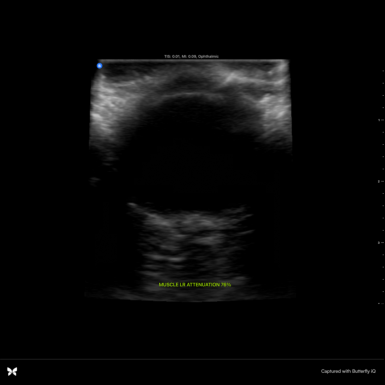
\includegraphics[width=0.3\textwidth]{images/uncropped.png}
    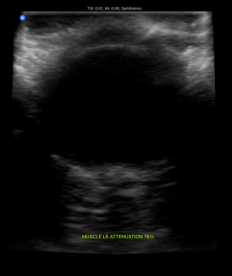
\includegraphics[width=0.3\textwidth]{images/cropped.png}
\end{center}

\section*{Challenges}


\section*{Approach}


\section*{Evaluation and Summary}


\section*{What I Learned}


\bibliographystyle{IEEEtran}
\bibliography{bibliography}

\end{document}